%% Definición de variables
\newcommand{\totalStudies}{114}
\newcommand{\databaseStudies}{99}
\newcommand{\snowballStudies}{14}
%Que yo recuerde en nuestro trabajo aún no hicimos inclusión directa de trabajos, sin embargo lo coloco aquí para el futuro.
\newcommand{\directInclusionStudies}{0}



% subseccion 4.2 ------- BUSQUEDA DE ESTUDIOS.
\subsection{Etapa 2: Búsqueda de Estudios}

Esta etapa presenta la estrategia de búsqueda utilizada en el SMS. Esta estrategia será definida y descrita en detalle en las subsecciones~\ref{subsubsec:estrategia-busqueda}--\ref{subsubsec:resultados-busqueda}. Ver Figura \ref{fig:busqueda-estudios}.
El resultado de esta etapa fue \totalStudies{} estudios obtenidos de esta manera. Hubo \databaseStudies{} estudios por bases de datos y  \snowballStudies{} estudios por bola de nieve.


% -------- Tabla : Actividades de la etapa de búsqueda de estudios. ------------
\begin{figure}[htbp]
	\centering
	\vspace{10pt}
	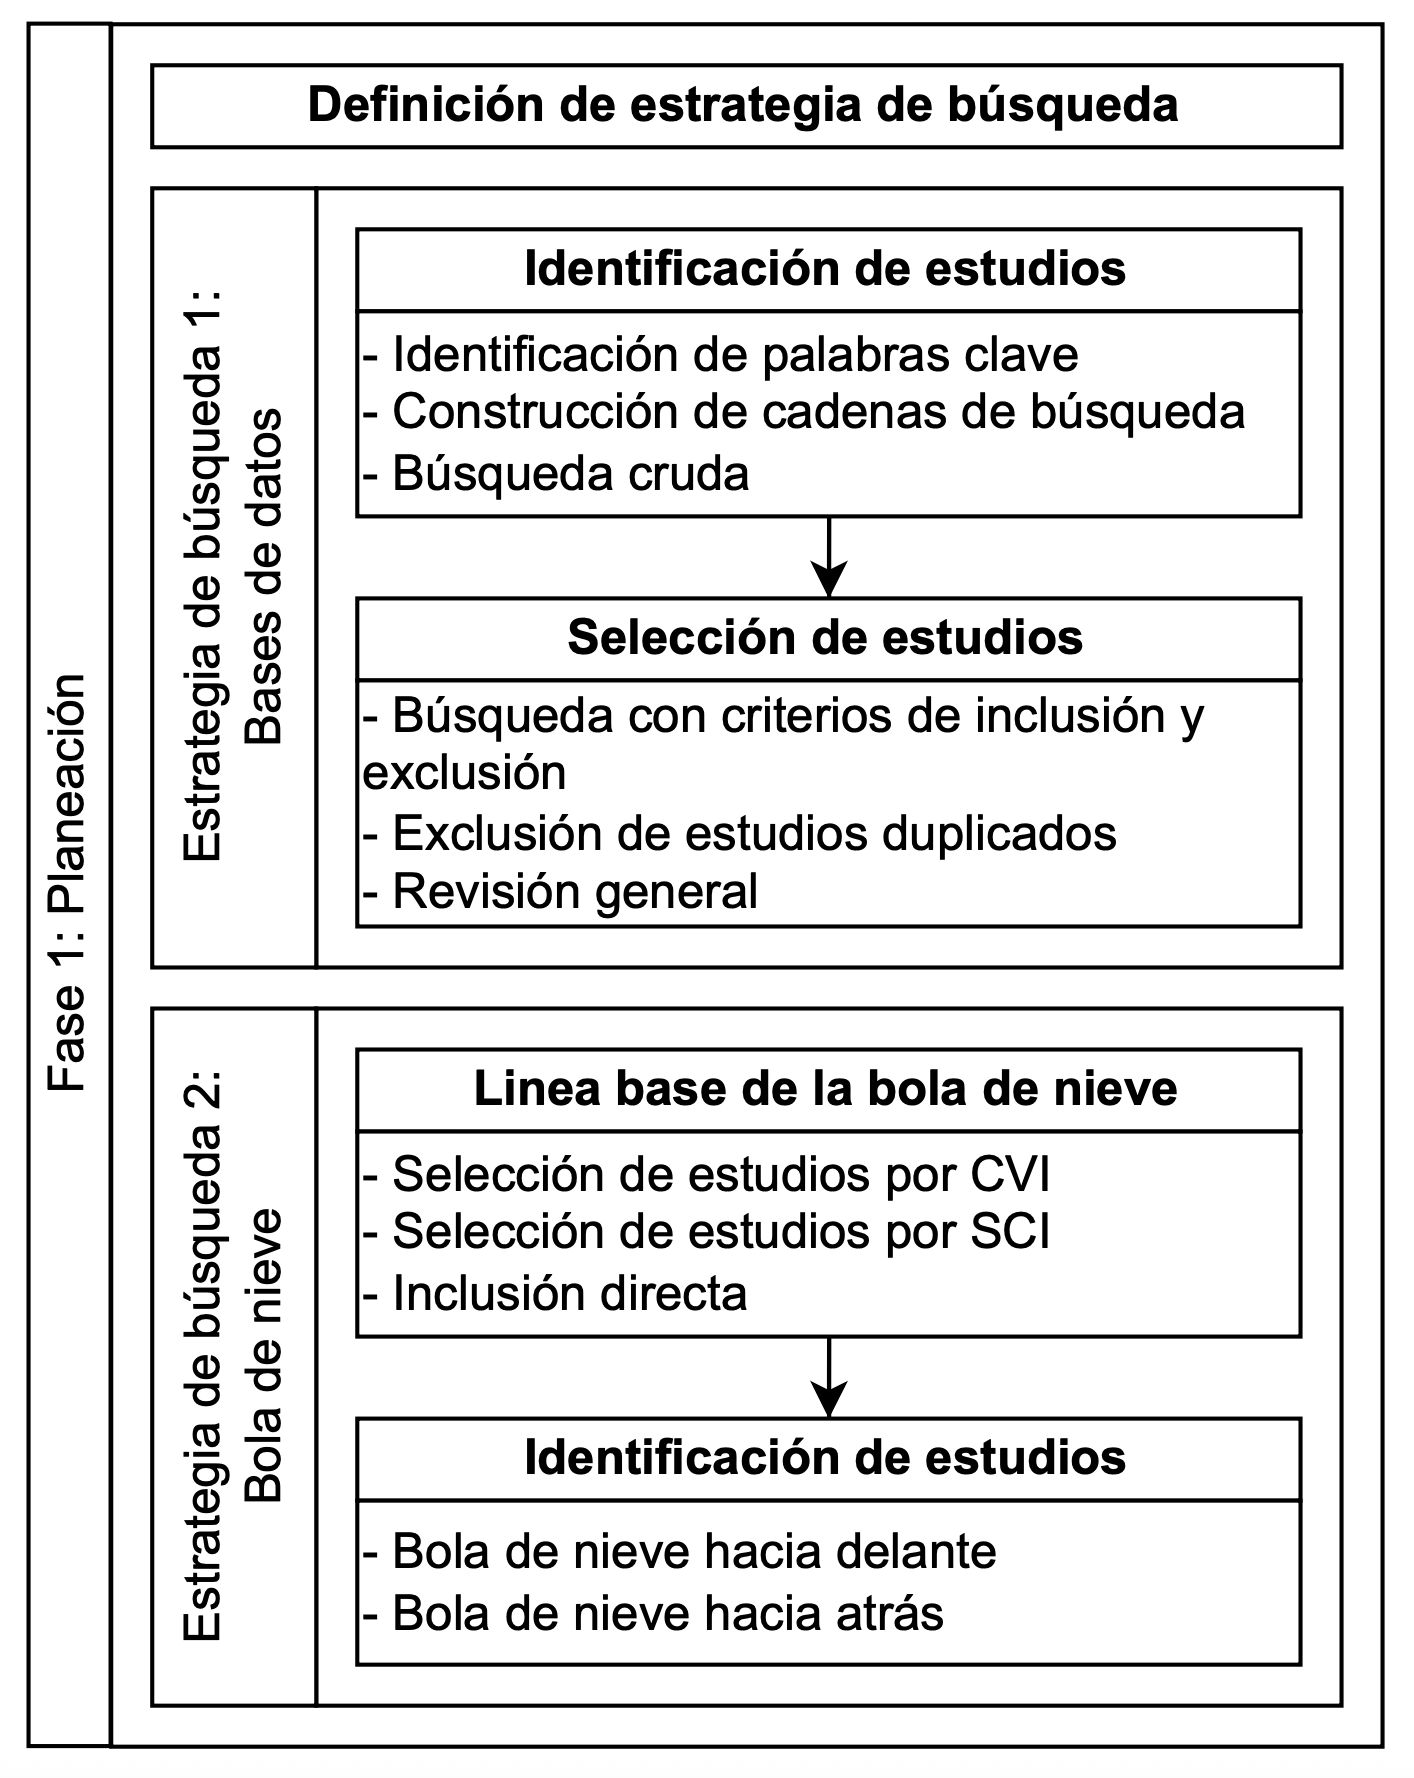
\includegraphics[scale=0.33]{resources/figures/fig03-fase1-planeacion.png}
	\caption{Actividades de la etapa de búsqueda de estudios.}
	\label{fig:busqueda-estudios}
\end{figure}

%sub-subseccion 4.2.1 ------ DEFINICIÓN DE ESTRATEGIA.
%sub-subseccion 4.2.1 
\subsubsection{Definiendo la Estrategia de Búsqueda}\label{subsubsec:estrategia-busqueda}

Para desarrollar este SMS, hemos implementado una metodología híbrida. Esta metodología tiene como objetivo conseguir una cantidad más
amplia de estudios indexados y procedentes de múltiples fuentes, superando los resultados que ofrecen en las bases de datos. De esta manera, integramos dos técnicas de búsqueda. La técnica inicial se denomina ``Búsqueda en bases de datos'' la cual consiste en realizar una búsqueda automatizada dentro de bases de datos académicas indexadas~\cite{Jalai-01}. La técnica secundaria recibe el
nombre de \textit{Snowballing} o  \textit{bola de nieve} y representa un procedimiento manual fundamentado en una  previa recolección de textos iniciales para
identificar investigaciones adicionales mediante sus bibliografías y citaciones~\cite{Jalai-01,Goodman-01}.

Para apoyar el proceso llevado a cabo en este SMS, hemos utilizado los siguientes elementos: a) Bases de datos académicas. b) El software SMS-Builder desarrollado por Candela et al.~\cite{sms-builder-repo} diseñado específicamente para facilitar la construcción de estudios de mapeo sistemático. c) Herramientas para apoyar la gestión de referencias como Mendeley y Google Scholar. %Aquí omití EndNote porque pues no lo usamos.


%sub-subseccion 4.2.2 ----- BUSQUEDA POR BASES DE DATOS 

%%% Variables de frecuencia por cada base de datos. 
\newcommand{\acm}{518}
\newcommand{\ieee}{0}
\newcommand{\sd}{120}
\newcommand{\spr}{209}
\newcommand{\tf}{0}
\newcommand{\tot}{847}
%%% Variables de contrubución porcetual
\newcommand{\acmp}{\fpeval{round(\acm*100/\tot,2)}}
\newcommand{\ieeep}{\fpeval{round(\ieee*100/\tot,2)}}
\newcommand{\sdp}{\fpeval{round(\sd*100/\tot,2)}}
\newcommand{\sprp}{\fpeval{round(\spr*100/\tot,2)}}
\newcommand{\tfp}{\fpeval{round(\tf*100/\tot,2)}}

%%%%% ------------------------------------------------

%%% Variables de frecuencia por cada base de datos. 
\newcommand{\iacm}{315}
\newcommand{\iieee}{0}
\newcommand{\isd}{101}
\newcommand{\ispr}{63}
\newcommand{\itf}{0}
\newcommand{\itot}{479}
%%% Variables de contribución porcentual
\newcommand{\iacmp}{\fpeval{round(\iacm*100/\itot,2)}}
\newcommand{\iieeep}{\fpeval{round(\iieee*100/\itot,2)}}
\newcommand{\isdp}{\fpeval{round(\isd*100/\itot,2)}}
\newcommand{\isprp}{\fpeval{round(\ispr*100/\itot,2)}}
\newcommand{\itfp}{\fpeval{round(\itf*100/\itot,2)}}

%Cantidad de estudios excluídos por ser duplicados
\newcommand{\numEstEx}{3}

%Cantidad de estudios luego de depuración = (estudios totales luego de exclusión - estudios duplicados)
\newcommand{\depTot}{\fpeval{\itot-\numEstEx}}

%Cantidad de estudios depurados por el screening
\newcommand{\screen}{377}
%Cantidad de estudios totales luego del screening
\newcommand{\screenTot}{\fpeval{\depTot-\screen}}

%sub-subseccion 4.2.2
\subsubsection{Search Strategy 1: Databases}

This strategy comprises two components. The first component is termed ``Study Identification''. It focuses on establishing the keywords to construct search strings that enable the completion of queries in digital libraries. The second component is called ``Study Selection''. It focuses on applying various criteria to refine study search results and select those with the most significant value for the SMS\@

\bolditalic{Study Identification}: in order to ensure the feasibility of the SMS and by consensus of the authors, it was decided to limit the number of databases to five, including ACM, IEEE Xplore, Springer, ScienceDirect, Taylor \& Francis. In this part of the process, it is necessary to establish the keywords used subsequently in the search strings for each of the databases. Again, we used the PICOC model as a methodological guide to identify key terms or phrases that serve this purpose. We refined these terms by including synonyms (See Table~\ref{table:picoc_keywords}).

% -------- Table : Keywords identified using PICOC model. ------------
\begin{table}[htbp]
	\centering
	\caption{Keywords identified using the PICOC model}
	\label{table:picoc_keywords}
	\renewcommand{\arraystretch}{1}  % Increase row height globally
	\begin{tabular}{p{1.8cm}p{6cm}}
		\toprule
		\textbf{Component}           & \textbf{Keywords}                                                                                                                                                                                                                                                    \\
		\midrule
		\textbf{Population}          & Universes, HTCondor, Distributed and parallel computing, HTC, Software development, Virtualization and microservices, Computer networks, Computational infrastructure, Artificial intelligence, Data analysis, Computational thinking, Research, Teaching, Industry. \\
		\addlinespace[0.8em]
		\textbf{Intervention}        & Identification and classification.                                                                                                                                                                                                                                   \\
		\addlinespace[0.8em]
		\textbf{Acceptance Criteria} &
		Documented project cases, compliance with inclusion and exclusion criteria, and appearance in selected databases.                                                                                                                                                                                   \\
		\addlinespace[0.8em]
		\textbf{Outcomes}            & Taxonomy that organizes works related to the population.                                                                                                                                                                                                             \\
		\addlinespace[0.8em]
		\textbf{Context}             & HTCondor universes, distributed and parallel computing domains, academic functions, research, teaching, industry.                                                                                                                                                    \\
		\bottomrule
	\end{tabular}
\end{table}
% --------------------------------------------------------------


The selected main keywords were \textit{HTCondor, HTC, Universe, Project, Research}. To broaden the research perspective, we used the Boolean operator ``OR'' to add synonyms to the main keywords.

Finally, the set of keywords selected for the construction of the search string are found in Table~\ref{table:database_search_keywords}.


% -------- Table : Keywords for database search ------------
\begin{table}[htbp]
	\centering
	\caption{Keywords for database search}
	\label{table:database_search_keywords}
	\renewcommand{\arraystretch}{1}  % Increase row height globally
	\begin{tabular}{p{1.4cm}p{6.4cm}}
		\toprule
		\textbf{Keyword}  & \textbf{Synonyms and related concepts}                     \\
		\midrule
		\textbf{HTCondor} & Condor                                                     \\
		\addlinespace[0.8em]
		\textbf{HTC}      & HPC, High Throughput Computing, High Performance Computing \\
		\addlinespace[0.8em]
		\textbf{Universe} & Execution Environment                                      \\
		\addlinespace[0.8em]
		\textbf{Project}  & Work                                                       \\
		\addlinespace[0.8em]
		\textbf{Research} & Teaching, Industry                                         \\
		\bottomrule
	\end{tabular}
\end{table}
% --------------------------------------------------------------





% -------- Table : Search strings used in databases ------------
\begin{table*}[htbp]
	\centering
	\caption{Search strings used in databases}
	\label{table:cadenas_de_busqueda}
	\renewcommand{\arraystretch}{1}  % Increase row height globally
	\begin{tabular}{p{3.2cm}p{11cm}p{2.5cm}}
		\toprule
		\textbf{Database}                 & \textbf{Search String}                                                                                                                                                                                              & \textbf{Fields} \\
		\midrule
		\textbf{ACM Full Text Collection} & ((HTCondor OR Condor) AND (HTC OR ``High Throughput Computing'' OR HPC OR ``High Performance Computing'') AND (Universe OR ``Execution Environment'') AND (Project OR Work) AND (Research OR Teaching OR Industry)) & All fields      \\
		\addlinespace[0.8em]
		\textbf{IEEE Xplore}              & ((HTCondor OR Condor) AND (HTC OR ``High Throughput Computing'' OR HPC OR ``High Performance Computing'') AND (Universe OR ``Execution Environment'') AND (Project OR Work) AND (Research OR Teaching OR Industry)) & All fields      \\
		\addlinespace[0.8em]
		\textbf{Springer}                 & ((HTCondor | Condor) + (HTC | ``High Throughput Computing'' | HPC | ``High Performance Computing'') + (Universe | ``Execution Environment'') + (Project | Work) + (Research | Teaching | Industry))                 & All fields      \\
		\addlinespace[0.8em]
		\textbf{ScienceDirect}            & (HTCondor OR Condor) (HTC OR ``High Throughput Computing'' OR HPC OR ``High Performance Computing'') (Universe OR ``Execution Environment'') (Project OR Work) (Research OR Teaching OR Industry)                   & All fields      \\
		\addlinespace[0.8em]
		\textbf{Taylor \& Francis}        & ((HTCondor OR Condor) AND (HTC OR ``High Throughput Computing'' OR HPC OR ``High Performance Computing'') AND (Universe OR ``Execution Environment'') AND (Project OR Work) AND (Research OR Teaching OR Industry)) & All fields      \\
		\bottomrule
	\end{tabular}
\end{table*}
% --------------------------------------------------------------


To direct the research toward the intersection of these two groups of terms, the Boolean operator ``AND'' was used. Once we identified the keywords, we continued constructing the search strings for the digital libraries using an iterative process. The iterative construction of search strings consists of performing a heuristic process with keywords, synonyms, and related concepts through the use of disjunctions and conjunctions that conform to the syntactic rules of each database considered in the automated search. Therefore, these strings vary according to the characteristics and functions of each database. See Table~\ref{table:cadenas_de_busqueda}.

After constructing the search strings, these were submitted to each database engine. Table~\ref{table:search_results} shows the set of results obtained. We identified a total of 847 studies preliminarily, with ACM being the largest contributor, delivering the greatest number of results compared to the other databases with \acmp\% of the results.


\begin{table*}[htbp]
	\centering
	\caption{Search string results}
	\label{table:search_results}
	\renewcommand{\arraystretch}{1}  % Increase row height globally
	\begin{tabular}{p{4.8cm}p{1.7cm}p{1.7cm}p{1.7cm}p{1.7cm}p{2cm}p{1.4cm}}
		\toprule
		\textbf{Criteria}                         & \textbf{ACM} & \textbf{IEEE} & \textbf{ScienceDirect} & \textbf{Springer} & \textbf{Taylor\&Francis} & \textbf{Total} \\
		\midrule
		\textbf{Search string with keywords only} & \acm{}       & \ieee{}       & \sd{}                  & \spr{}            & \tf{}                    & \tot{}         \\
		\addlinespace[0.8em]
		\textbf{Percentage contribution}          & \acmp{}\%    & \ieeep{}\%    & \sdp{}\%               & \sprp{}\%         & \tfp{}\%                 & 100\%          \\
		\bottomrule
	\end{tabular}
\end{table*}
% --------------------------------------------------------------




\bolditalic{Study Selection}: to refine the results obtained up to this point, we applied the inclusion and exclusion criteria defined in the planning stage. Table~\ref{table:search_results_exclusion} shows the results of this step. After applying said filter, the total number of studies obtained was \itot. According to the different databases consulted, ACM continues to have the most considerable contribution, with \iacmp\% of the studies.

%% Applying duplicate exclusion

From the \itot{} studies selected, the exclusion of three studies was applied given that these were duplicates. After this refinement, the total studies were \depTot{}. From this new dataset, a review named \bolditalic{screening} was conducted, this procedure consists of verifying the title, abstract, and keywords of each study to determine if these are circumscribed within the research context, that is, if they are aligned with the objectives proposed for the SMS. The \textit{screening} process allowed us to discard \screen{} studies given that some of them made reference to different academic disciplines and others were not aligned with the research objectives proposed.

Therefore, we concluded the first search strategy with a total of \screenTot{} studies selected. Figure~\ref{fig:overview} shows an overview of the activities and results obtained in search strategy 1.

\begin{figure}[htbp]
	\centering
	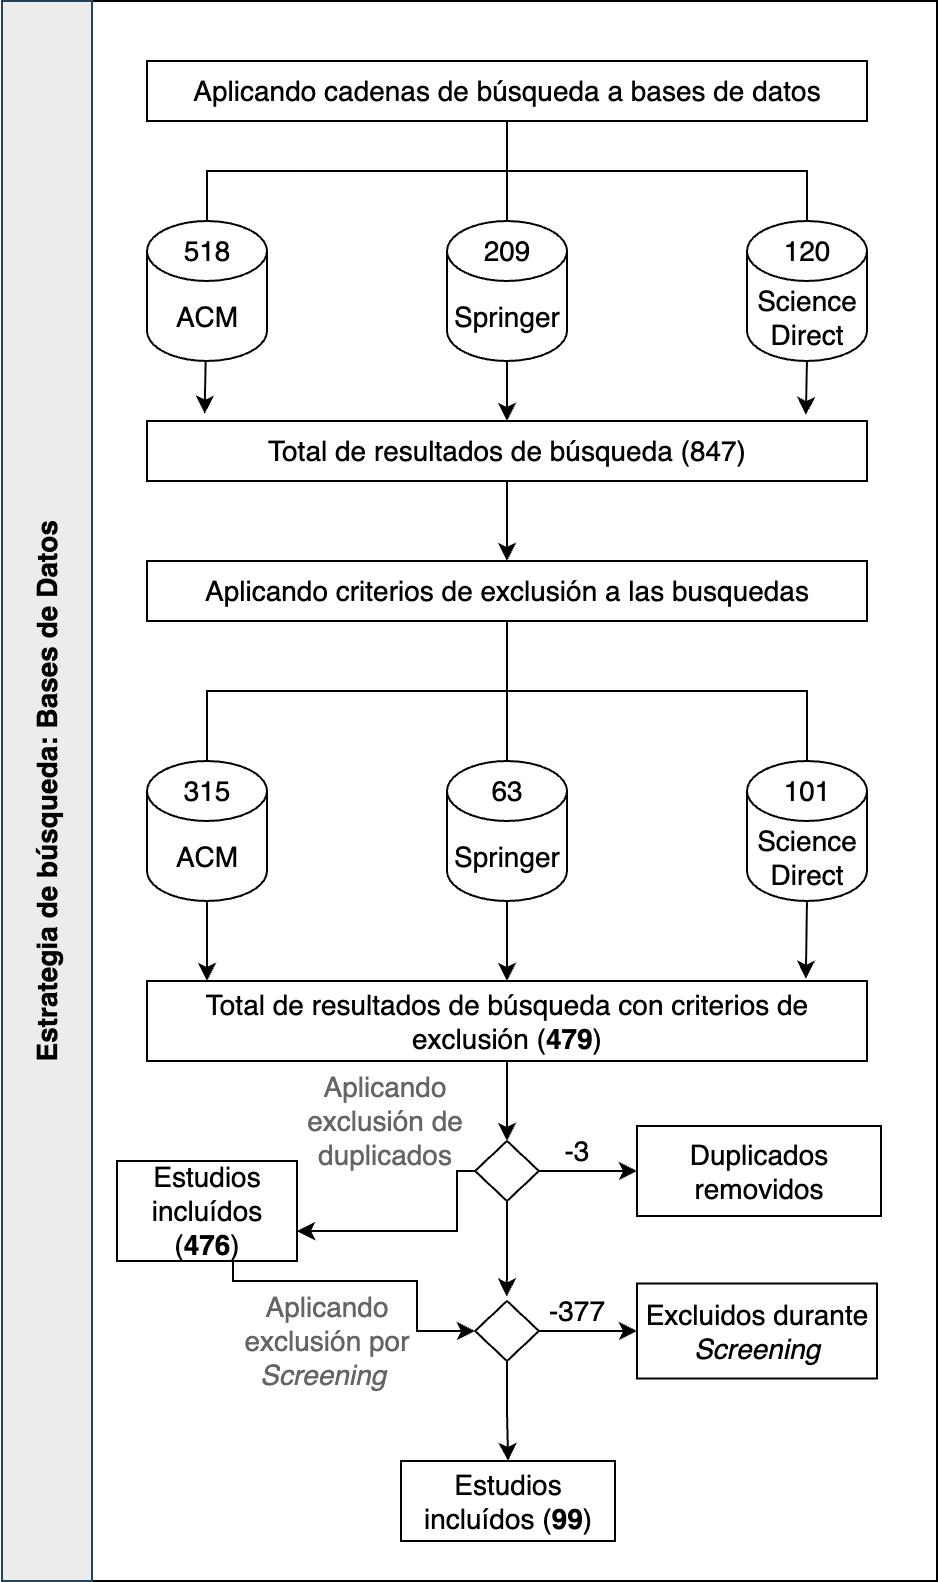
\includegraphics[scale=0.25]{resources/figures/overview.png}
	\caption{Overview of activities and results obtained in the database search strategy}
	\label{fig:overview}
\end{figure}


\begin{table*}[htbp]
	\centering
	\caption{Search string results with exclusion/inclusion criteria}
	\label{table:search_results_exclusion}
	\begin{tabular}{p{4.8cm}p{1.7cm}p{1.7cm}p{1.7cm}p{1.7cm}p{2cm}p{1.4cm}}
		\toprule
		\textbf{Criteria}                         & \textbf{ACM} & \textbf{IEEE} & \textbf{ScienceDirect} & \textbf{Springer} & \textbf{Taylor \& Francis} & \textbf{Total} \\
		\midrule
		\textbf{Search string with keywords only} & \iacm{}      & \iieee{}      & \isd{}                 & \ispr{}           & \itf{}                     & \itot{}        \\
		\addlinespace[0.8em]
		\textbf{Percentage contribution}          & \iacmp{}\%   & \iieeep{}\%   & \isdp{}\%              & \isprp{}\%        & \itfp{}\%                  & 100\%          \\
		\bottomrule
	\end{tabular}
\end{table*}
% --------------------------------------------------------------




% sub-subsetion for 4.2.3 --- BUSQUEDA POR SNOWBALL 
% sub-subsetion for 4.2.3 ----- ESTRATEGIA DE BUSQUEDA POR SNOWBALL
\subsubsection{Estrategia de Búsqueda 2: Bola de Nieve (Snowballing)}

\newcommand{\csiSelected}{24} %Estudios identficados con el SCI
\newcommand{\newSnowballStudies}{3} %Estudios obtenidos luego de aplicar criterios de inclusión y exclusión diseñados especificamente para el snowball.
\newcommand{\firstBackwardSnowballStudies}{3} %Primera iteración hacia atrás
\newcommand{\firstForwardSnowballStudies}{4} % Primera iteración hacia adelante
\newcommand{\secondBackwardSnowballStudies}{3} %Segunda iteracion haia atrás
\newcommand{\secondForwardSnowballStudies}{5} %Segunda iteración hacia adelante

%Total primer iteración.
\newcommand{\firstSnowballIterationStudies}{\fpeval{\firstBackwardSnowballStudies+\firstForwardSnowballStudies}}
%Total segunda iteración.
\newcommand{\secondSnowballIterationStudies}{\fpeval{\secondBackwardSnowballStudies+\secondForwardSnowballStudies}}

\newcommand{\snowballNewStudies}{\fpeval{\firstSnowballIterationStudies+\secondSnowballIterationStudies}}

La estrategia de búsqueda por bola de nieve comienza con la identificación del conjunto base de documentos a utilizar, seguido de una revisión y selección de documentos. La revisión consiste en verificar la lista de referencias con el fin de identificar nuevos documentos (bola de nieve hacia atrás). De manera similar, se identifican los documentos que citan el documento revisado (bola de nieve hacia adelante), lo cual requiere el uso de un buscador que indique esta información; para dicho fin se hizo uso de Google Scholar. En todos los casos, la sección de documentos aplica los criterios de exclusión \cite{Wohlin-01}.

Esta estrategia comprende dos pasos. El primer paso se denomina ``Construcción de línea base de bola de nieve'' y se enfoca en establecer estudios para iniciar el análisis de referencias y citas. Para la composición de este conjunto de estudios, utilizamos criterios basados en el SCI (Índice de Citas de Estudios). El segundo paso se denomina ``Selección de estudios'', y se enfoca en el análisis de referencias (Bola de nieve hacia atrás) y citas (Bola de nieve hacia adelante) de cada estudio.


% Snowball baseline building 

\bolditalic{Construcción de línea base de bola de nieve}: Basándonos en los \screenTot{} estudios seleccionados durante la fase de \textit{screening}, se realizó un análisis exhaustivo de frecuencia y relevancia académica mediante el cual se evaluó la calidad e impacto científico de cada publicación.

A través de la aplicación sistemática del índice SCI como criterio de selección por calidad, se logró identificar y extraer \csiSelected{} estudios de alta relevancia que constituyen la base fundamental para la implementación de la estrategia de búsqueda por bola de nieve. Luego, se aplicaron los criterios de inclusión y exclusión propuestos en la Tabla \ref{table:inclusion_exclusion_criteria} para limitar la cantidad de estudios a los más recientes según el período de publicación, con esto se logró disminuir a \newSnowballStudies{} la cantidad de estudios semilla de la bola de nieve.

Estos últimos estudios, caracterizados por su alto índice de citación y reconocimiento en la comunidad científica, servirán como punto de partida para las iteraciones de \textit{snowball} hacia adelante (\textit{forward snowballing}, esto es, aquellos trabajos que citaron nuestros estudios base) y hacia atrás (\textit{backward snowballing}, es decir, aquellos trabajos citados en nuestros estudios base), permitiendo así expandir la búsqueda bibliográfica de manera dirigida en el dominio de los universos HTCondor.


\bolditalic{Selección de estudios}: Para esta actividad se decidió hacer dos iteraciones de bola de nieve. Se comienza con la primera iteración revisando que estudios citaron y que estudios fueron citados por cada uno de los \newSnowballStudies{} estudios semilla. Esta revisión permitió identificar \firstSnowballIterationStudies{} nuevos artículos que cumplen con nuevos criterios de inclusión y exclusión fabricados para este proceso. Luego, se procede con la segunda iteración de la bola de nieve, la cual se aplica para cada uno de los \firstSnowballIterationStudies{} estudios extraídos en la primera iteración. Esta revisión permitió identificar otros \secondSnowballIterationStudies{} nuevos estudios para ser incluidos en el SMS. Ver Figura \ref{figure:Snowball}.\\

\begin{figure}[htbp]
	\centering
	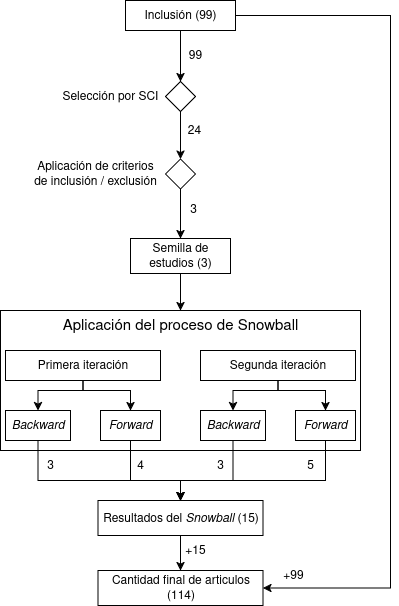
\includegraphics[scale=0.55]{resources/figures/sms-Snowball.drawio.png}
	\caption{Estrategia de búsqueda por bola de nieve.}
	\label{figure:Snowball}
\end{figure}

Esta actividad se realizó a través de Google Scholar y siguiendo la práctica en el estudio \cite{Ali-01}. El resultado conseguido fueron \snowballNewStudies{} nuevos estudios. Cabe recalcar que lo presentado en esta sección y en la Figura \ref{figure:Snowball} es un resumen representativo del proceso de \textit{snowball}, sin embargo, se omiten pasos que se realizaron pero no aportan al objetivo del estudio.

% -------- Tabla : Criterios de inclusión/exclusión ------------
\begin{table}[htbp]
	\centering
	\caption{Criterios de inclusión/exclusión}
	\label{table:inclusion_exclusion_criteria}
	\renewcommand{\arraystretch}{1}  % Increase row height globally
	\begin{tabular}{p{1.5cm}p{2.2cm}p{3.9cm}}
		\toprule
		\textbf{Categoría}           & \textbf{Inclusión}         & \textbf{Exclusión}                                                                                                          \\
		\midrule
		\textbf{Tipo de publicación} & Artículos de investigación & Tesis, capítulos de libros, libros, revistas, conferencias, y todo lo demás que no esté en el tipo de publicación inclusiva \\
		\addlinespace[0.8em]
		\textbf{Período}             & Desde 2020 hasta 2024      & -                                                                                                                           \\
		\addlinespace[0.8em]
		\textbf{Idioma}              & Inglés                     & -                                                                                                                           \\
		\bottomrule
	\end{tabular}
\end{table}
% --------------------------------------------------------------



% sub-subsetion for 4.2.4 -- RESULTADOS DE LA BUSQUEDA DE ESTUDIOS
% sub=-subsection 4.2.4
\subsubsection{Resultados de la Búsqueda de Estudios}\label{subsubsec:resultados-busqueda}

Finalmente, añadiendo los \snowballNewStudies{} estudios obtenidos en el proceso de bola de nieve a los \screenTot{} previamente obtenidos con la estrategia de búsqueda por base de datos, se obtiene un total de 114 estudios para esta etapa.



